\documentclass[a4paper]{article}
\usepackage{tikz}
\usepackage{geometry}
\usepackage{graphicx}
\usepackage{natbib}
\usepackage{amsmath}
\usepackage{amssymb}
\usepackage{amsthm}
\usepackage{paralist}
\usepackage{epstopdf}
\usepackage{tabularx}
\usepackage{longtable}
\usepackage{multirow}
\usepackage{multicol}
\usepackage[hidelinks]{hyperref}
\usepackage{fancyvrb}
\usepackage{algorithm}
\usepackage{algorithmic}
\usepackage{float}
\usepackage{paralist}
%\usepackage[svgname]{xcolor}
\usepackage{enumerate}
\usepackage{array}
\usepackage{times}
\usepackage{url}
\usepackage{fancyhdr}
\usepackage{comment}
\usepackage{environ}
\usepackage{times}
\usepackage{textcomp}
\usepackage{caption}
\usepackage{bbm}



\urlstyle{rm}

\setlength\parindent{0pt} % Removes all indentation from paragraphs
\theoremstyle{definition}
\newtheorem{definition}{Definition}[]
\newtheorem{conjecture}{Conjecture}[]
\newtheorem{example}{Example}[]
\newtheorem{theorem}{Theorem}[]
\newtheorem{lemma}{Lemma}
\newtheorem{proposition}{Proposition}
\newtheorem{corollary}{Corollary}

\floatname{algorithm}{Procedure}
\renewcommand{\algorithmicrequire}{\textbf{Input:}}
\renewcommand{\algorithmicensure}{\textbf{Output:}}
\newcommand{\abs}[1]{\lvert#1\rvert}
\newcommand{\norm}[1]{\lVert#1\rVert}
\newcommand{\RR}{\mathbb{R}}
\newcommand{\CC}{\mathbb{C}}
\newcommand{\Nat}{\mathbb{N}}
\newcommand{\br}[1]{\{#1\}}
\DeclareMathOperator*{\argmin}{arg\,min}
\DeclareMathOperator*{\argmax}{arg\,max}
\renewcommand{\qedsymbol}{$\blacksquare$}

\definecolor{dkgreen}{rgb}{0,0.6,0}
\definecolor{gray}{rgb}{0.5,0.5,0.5}
\definecolor{mauve}{rgb}{0.58,0,0.82}

\definecolor{C0}{HTML}{1F77B4}
\definecolor{C1}{HTML}{FF7F0E}
\definecolor{C2}{HTML}{2ca02c}
\definecolor{C3}{HTML}{d62728}
\definecolor{C4}{HTML}{9467bd}
\definecolor{C5}{HTML}{8c564b}
\definecolor{C6}{HTML}{e377c2}
\definecolor{C7}{HTML}{7F7F7F}
\definecolor{C8}{HTML}{bcbd22}
\definecolor{C9}{HTML}{17BECF}

\newcommand{\Var}{\mathrm{Var}}
\newcommand{\Cov}{\mathrm{Cov}}
\newcommand{\sgn}{\mathrm{sgn}}

\newcommand{\vc}[1]{\boldsymbol{#1}}
\newcommand{\xv}{\vc{x}}
\newcommand{\Sigmav}{\vc{\Sigma}}
\newcommand{\alphav}{\vc{\alpha}}
\newcommand{\muv}{\vc{\mu}}

\newcommand{\red}[1]{\textcolor{red}{#1}}

\def\x{\mathbf x}
\def\y{\mathbf y}
\def\w{\mathbf w}
\def\v{\mathbf v}
\def\E{\mathbb E}
\def\R{\mathbb R}
\def\V{\mathbb V}
\def\ind{\mathbbm 1}

% TO SHOW SOLUTIONS, include following (else comment out):
\newenvironment{soln}{
    \leavevmode\color{blue}\ignorespaces
}{}


\hypersetup{
%    colorlinks,
    linkcolor={red!50!black},
    citecolor={blue!50!black},
    urlcolor={blue!80!black}
}

\geometry{
  top=1in,            % <-- you want to adjust this
  inner=1in,
  outer=1in,
  bottom=1in,
  headheight=3em,       % <-- and this
  headsep=2em,          % <-- and this
  footskip=3em,
}


\pagestyle{fancyplain}
\lhead{\fancyplain{}{Homework 7}}
\rhead{\fancyplain{}{CS 760 Machine Learning}}
\cfoot{\thepage}

\title{\textsc{Homework 7}} % Title

%%% NOTE:  Replace 'NAME HERE' etc., and delete any "\red{}" wrappers (so it won't show up as red)

\author{
\red{$>>$Martin Diges$<<$} \\
\red{$>>$9080689699$<<$}\\
} 

\date{}

\begin{document}

\maketitle 

\textbf{Instructions:}
Use this latex file as a template to develop your homework. Please submit a single pdf to Canvas. Late submissions may not be accepted. You can choose any programming language (i.e. python, R, or MATLAB). Please check Piazza for updates about the homework.
\vspace{0.1in}
\\\\
% \hypersetup{colorlinks=true, linkcolor=cyan}
\url{https://github.com/missingnoglitch0/cs760/tree/main/hw7}

\section{Getting Started}
Before you can complete the exercises, you will need to setup the code.
%
In the zip file given with the assignment, there is all of the starter code you will need to complete it.
%
You will need to install the requirements.txt where the typical method is through python's virtual environments.
%
Example commands to do this on Linux/Mac are:
\begin{verbatim}
    python -m venv .venv
    source .venv/bin/activate
    pip install -r requirements.txt 
\end{verbatim}
%

For Windows or more explanation see here: \url{https://docs.python.org/3/tutorial/venv.html}

\section{Value Iteration [40 pts]}

The \verb|ValueIteration| class in \verb|solvers/Value_Iteration.py| contains the implementation for the value iteration algorithm. Complete the \verb|train_episode| and \verb|create_greedy_policy| methods.

\subsubsection*{Submission [6 pts each + 10 pts for code submission]}

Submit a screenshot containing your \verb|train_episode| and \verb|create_greedy_policy| methods (10 points).

\begin{figure}[H]
    \centering
    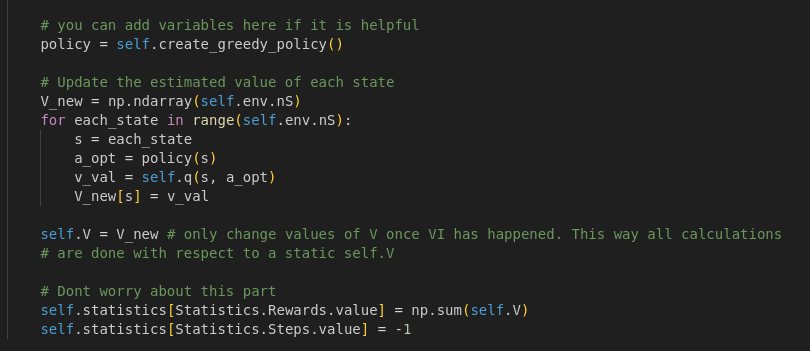
\includegraphics[width=6in]{2_train_episode.png}
    \caption{train\_episode()}
    \label{fig:gan_q1_loss}
\end{figure}

\begin{figure}[H]
    \centering
    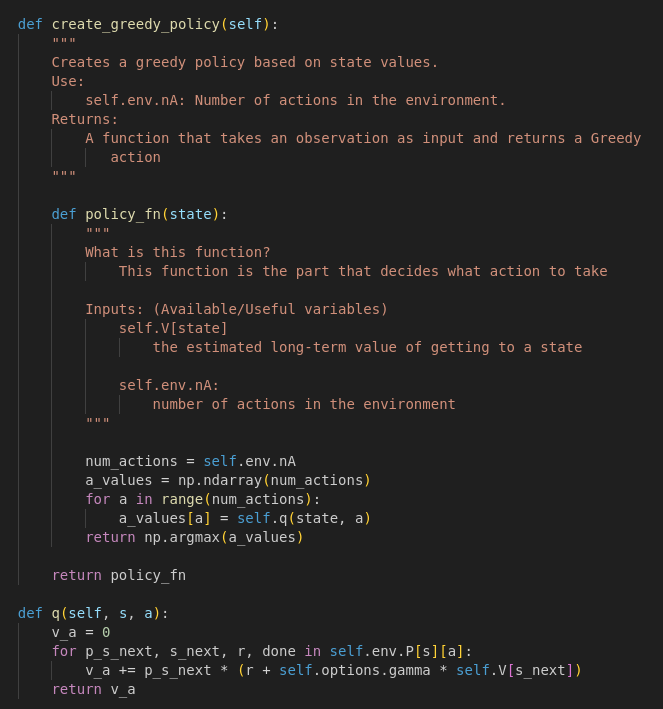
\includegraphics[width=6in]{2_create_greedy_policy.png}
    \caption{create\_greedy\_policy() and auxiliary function q()}
    \label{fig:gan_q1_loss}
\end{figure}


\vspace{5mm}
For these 5 commands. Report the episode it converges at and the reward it achieves. See examples for what we expect. An example is: \begin{verbatim}
    python run.py -s vi -d Gridworld -e 200 -g 0.2
\end{verbatim}
Converges to a reward of \verb|___| in \verb|___| episodes.

\red{Note: For FrozenLake the rewards go to many decimal places. Report convergence to the nearest 0.0001.}

\vspace{8mm}

Submission Commands:
\begin{enumerate} 
    \item   python run.py -s vi -d Gridworld -e 200 -g 0.05
            \\Converges to a reward of -14.51 in 3 episodes.
            
    \item   python run.py -s vi -d Gridworld -e 200 -g 0.2
            \\Converges to a reward of -16.16 in 3 episodes.
            
    \item  python run.py -s vi -d FrozenLake-v0 -e 500 -g 0.5
            \\(please see Piazza @336 for why the values below may differ from expected)
            \\Converges to a reward of 0.6374 in 14 episodes.
            
    \item  python run.py -s vi -d FrozenLake-v0 -e 500 -g 0.9 
            \\Converges to a reward of 2.1760 in 72 episodes. 
            
    \item python run.py -s vi -d FrozenLake-v0 -e 500 -g 0.75
            \\Converges to a reward of 1.1316 in 34 episodes.
\end{enumerate}
    

\subsubsection*{Examples}

For each of these commands. The expected reward is given for a correct solution. 
If your solution gives the same reward it doesn't guarantee correctness on the test cases that you report results on -- you're encouraged to develop your own test cases to supplement the provided ones.

\begin{verbatim}
      python run.py -s vi -d Gridworld -e 100 -g 0.9  
\end{verbatim}
Converges in 3 episodes with reward of -26.24.

\begin{verbatim}
      python run.py -s vi -d Gridworld -e 100 -g 0.4  
\end{verbatim}
Converges in 3 episodes with reward of -18.64.

\begin{verbatim}
      python run.py -s vi -d FrozenLake-v0 -e 100 -g 0.9  
\end{verbatim}
Achieves a reward of 2.176 after 53 episodes.

\section{Q-learning [40 pts]}

The \verb|QLearning| class in \verb|solvers\Q_Learning.py| contains the implementation for the Q-learning algorithm. Complete the \verb|train_episode|, \verb|create_greedy_policy|,  and \verb|make_epsilon_greedy_policy| methods.

\subsubsection*{Submission [10 pts each + 10 pts for code submission]}

Submit a screenshot containing your \verb|train_episode|, \verb|create_greedy_policy| and 

\verb|make_epsilon_greedy_policy| methods (10 points).

\begin{figure}[H]
    \centering
    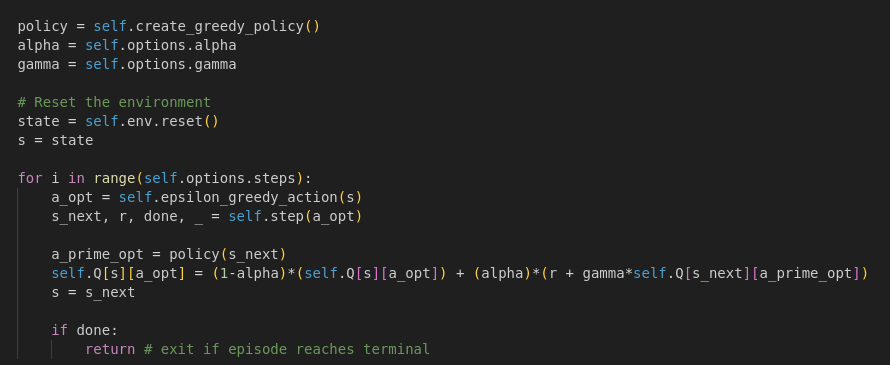
\includegraphics[width=6in]{3_train_episode.png}
    \caption{train\_episode()}
    \label{fig:gan_q1_loss}
\end{figure}

\begin{figure}[H]
    \centering
    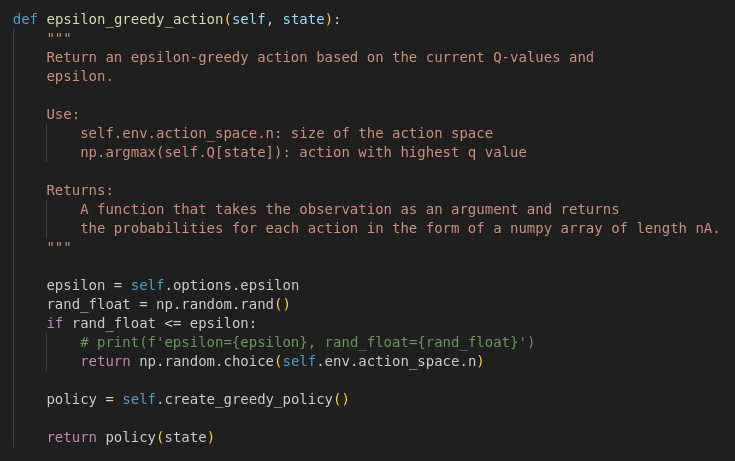
\includegraphics[width=6in]{3_make_epsilon_greedy_policy.png}
    \caption{make\_epsilon\_greedy\_policy()}
    \label{fig:gan_q1_loss}
\end{figure}

\begin{figure}[H]
    \centering
    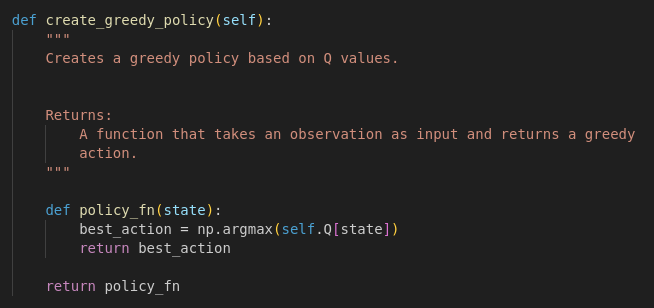
\includegraphics[width=6in]{3_create_greedy_policy.png}
    \caption{create\_greedy\_policy()}
    \label{fig:gan_q1_loss}
\end{figure}

\newpage
Report the reward for these 3 commands with your implementation (10 points each) by submitting the "Episode Reward over Time" plot for each command:

\begin{enumerate}
    \item  python run.py -s ql -d CliffWalking -e 100 -a 0.2 -g 0.9 -p 0.1
            \begin{figure}[H]
                \centering
                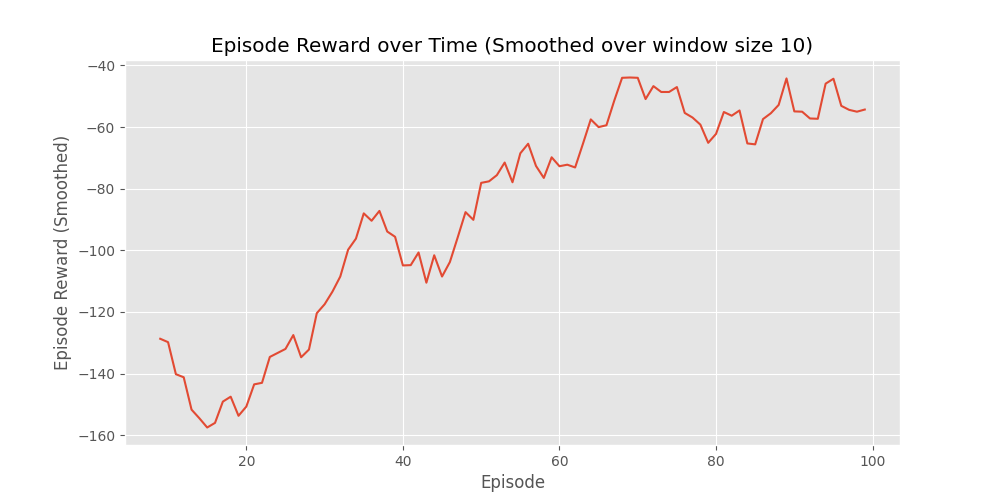
\includegraphics[width=6in]{3_1_EROT.png}
                % \caption{create\_greedy\_policy()}
                \label{fig:gan_q1_loss}
            \end{figure}
            
    \item  python run.py -s ql -d CliffWalking -e 100 -a 0.8 -g 0.5 -p 0.1  
            \begin{figure}[H]
                \centering
                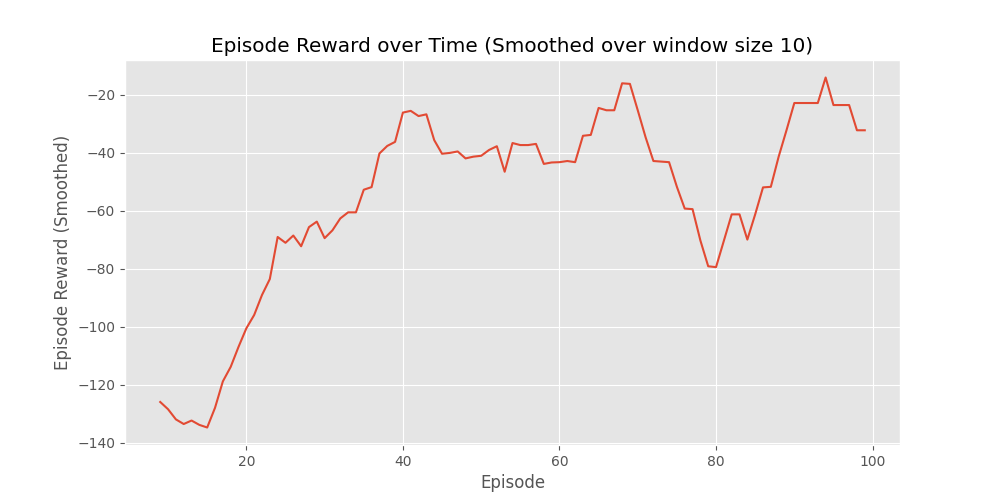
\includegraphics[width=6in]{3_2_EROT.png}
                % \caption{create\_greedy\_policy()}
                \label{fig:gan_q1_loss}
            \end{figure}
    
    \item  python run.py -s ql -d CliffWalking -e 500 -a 0.6 -g 0.8 -p 0.1   
            \begin{figure}[H]
                \centering
                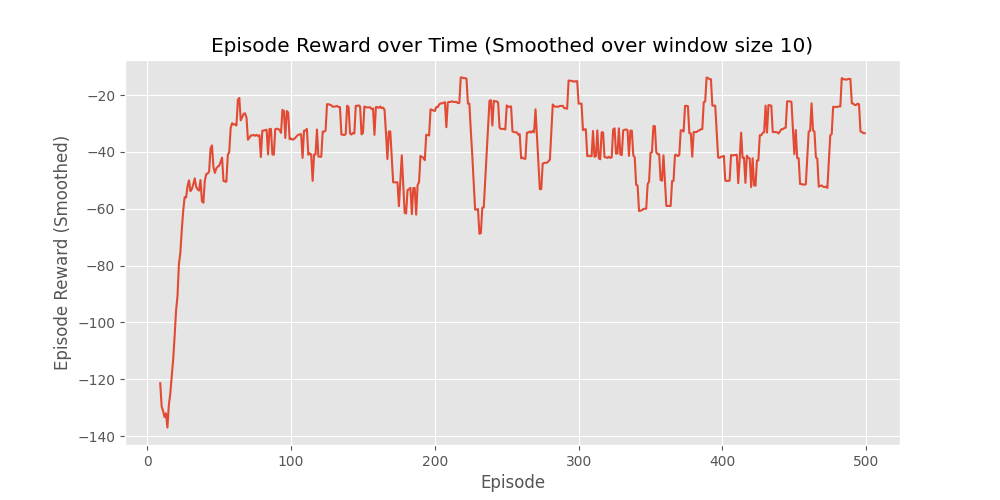
\includegraphics[width=6in]{3_3_EROT.png}
                % \caption{create\_greedy\_policy()}
                \label{fig:gan_q1_loss}
            \end{figure}
    
\end{enumerate}

For reference, command 1 should end with a reward around -60, command 2 should end with a reward around -25 and command 3 should end with a reward around -40.

\subsubsection*{Example}

Again for this command, the expected reward is given for a correct solution. If your solution gives the same reward it doesn't guarantee correctness on the test cases.

\begin{verbatim}
  python run.py -s ql -d CliffWalking -e 500 -a 0.5 -g 1.0 -p 0.1  
\end{verbatim}

Achieves a best performing policy with -13 reward.

\newpage
\section{Q-learning [20 pts]}
For this question you can either reimplement your Q-learning code or use your previous implementation. You will be using a custom made MDP for analysis. Consider the following Markov Decision Process.
It has two states $s$. It has two actions $a$: move and stay. The state transition is deterministic: ``move'' moves to the other state, while ``stay' stays at the current state. The reward $r$ is 0 for move,  1 for stay. There is a discounting factor $\gamma=0.8$.
\\

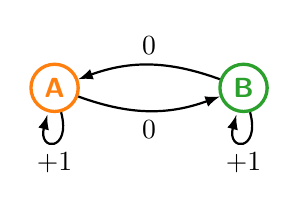
\begin{tikzpicture}
    \tikzstyle{n} = [very thick,circle,inner sep=0mm,minimum width=6mm]
    \tikzstyle{a} = [thick,>=latex,->]
    \def\dx{1.2}
    \def\dy{-1.2}
    \node[n,C1,draw=C1] (2) at (\dy,0) {\textbf{\textsf{A}}};
    \node[n,C2,draw=C2] (1) at (\dx,0) {\textbf{\textsf{B}}};
    \path[a]
    (2) edge [loop below] node {+1}(2)
    (1) edge [loop below] node {+1}(1)
    (2) edge [bend right=20] node[below] {0}(1)
    (1) edge [bend right=20] node[above] {0}(2);
\end{tikzpicture}

The reinforcement learning agent performs Q-learning.  Recall the $Q$ table has entries $Q(s,a)$. The $Q$ table is initialized with all zeros. The agent starts in state $s_1=A$. In any state $s_t$, the agent chooses the action $a_t$ according to a behavior policy $a_t = \pi_B(s_t)$. Upon experiencing the next state and reward $s_{t+1}, r_t$ the update is:
$$Q(s_t, a_t) \Leftarrow (1-\alpha) Q(s_t, a_t) + \alpha \left( r_t + \gamma \max_{a'} Q(s_{t+1}, a') \right).$$
Let the step size parameter $\alpha=0.5$.

\begin{enumerate}
\item (5 pts) Run Q-learning for 200 steps with a deterministic greedy behavior policy: at each state $s_t$ use the best action $a_t \in \argmax_a Q(s_t,a)$ indicated by the current action-value table. If there is a tie, prefer move. Show the action-value table at the end.
\\\{'A': \{'STAY': 0, 'MOVE': 0.0\}, 'B': \{'STAY': 0, 'MOVE': 0.0\}\}

\item (5 pts) Reset and repeat the above, but with an $\epsilon$-greedy behavior policy: at each state $s_t$, with probability $1-\epsilon$ choose what the current Q table says is the best action: $\argmax_a Q(s_t,a)$; Break ties arbitrarily. Otherwise, (with probability $\epsilon$) uniformly chooses between move and stay (move or stay both with 1/2 probability). Use $\epsilon=0.5$.
\\\{'A': \{'STAY': 4.999975828096329, 'MOVE': 3.687284964530014\}, 'B': \{'STAY': 4.700927716064728, 'MOVE': 3.999969476317586\}\}

\item (5 pts) Without doing simulation, use Bellman equation to derive the true action-value table induced by the MDP. That is, calculate the true optimal action-values by hand.

From the parameters supplied earlier, we have
$$Q(s_t, a_t) = (0.5) Q(s_t, a_t) + (0.5) \left( r_t + 0.8 \max_{a'} Q(s_{t+1}, a') \right)$$
$$Q(s_t, a_t) = \left( r_t + 0.8 \max_{a'} Q(s_{t+1}, a') \right)$$
$$Q(s_t, a_t) = \left( r_t + 0.8 \max (Q(s_{t+1}, STAY),Q(s_{t+1}, MOVE))  \right)$$
$$Q(s_t, STAY) = \left( 1 + 0.8 \max (Q(s_{t+1}, STAY),Q(s_{t+1}, MOVE)) \right)$$
$$Q(s_t, MOVE) = \left( 0 + 0.8 \max (Q(s_{t+1}, STAY),Q(s_{t+1}, MOVE)) \right)$$
It follows that $Q(s_t, STAY) > Q(s_t, MOVE)$. Since STAY is the max valued action, we have that
$$Q(s_t, STAY) = 1 + 0.8 Q(s_{t+1}, STAY)$$
$$Q(s_t, STAY) * (1-0.8) = 1$$
$$Q(s_t, STAY) = \frac{1}{1-0.8} = \frac{1}{0.2} = 5$$
and 
$$Q(s_t, MOVE) = 0 + 0.8 Q(s_{t+1}, STAY) = 0.8 (5) = 4$$

\item (5 pts) To the extent that you obtain different solutions for each question, explain why the action-values  differ.
\\For 1., We see that the action-value table retains its starting default values of 0 for all entries. This is because we explore deterministically and prefer to move when entires for stay and move are equal. Hence, we move and have a reward of 0. The updated action-values are always 0, so we keep moving and setting action-values to 0.
\\For 2., the $\epsilon$-greedy policy makes it more likely for random actions to be chosen and thus explored. This means the STAY action is sometimes chosen, leading to a $> 0$ action-value for each of our states. We thereby obtain nonzero action values.
\\In 3., we find the steady-state value for our $\epsilon$-greedy behavior, which is the set of values where applying our update rule would not lead to any changes in action-values.

\section{A2C (Extra credit)}
\subsection{Implementation}

You will implement a function for the A2C algorithm in solvers/A2C.py.
% 
Skeleton code for the algorithm is already provided in the relevant python files.
% 
Specifically, you will need to complete \verb|train| for A2C.
% 
To test your implementation, run:
% 
\begin{verbatim}
  python run.py -s a2c -t 1000 -d CartPole-v1 -G 200 
  
  -e 2000 -a\ 0.001 -g 0.95 -l [32]
\end{verbatim}
% 
This command will train a neural network policy with A2C on the CartPole domain for 2000 episodes.
% 
The policy has a single hidden layer with 32 hidden units in that layer.
\subsubsection*{Submission}
% 

For submission, plot the final reward/episode for 5 different values of either alpha or gamma. Then include a short (\verb|<5 sentence|) analysis on the impact that alpha/gamma had for the reward in this domain.



\end{enumerate}

\end{document}
